%----------------------------------------------------------------------------------------
%	PACKAGES AND DOCUMENT CONFIGURATIONS
%----------------------------------------------------------------------------------------

\documentclass{article}


\usepackage{graphicx} % Required for the inclusion of images
\graphicspath{{figures/}}
\usepackage{subfigure} % Required for the inclusion of images
\usepackage{natbib} % Required to change bibliography style to APA
\usepackage{amsmath} % Required for some math elements 
\usepackage{listings}
\usepackage{xcolor}
\usepackage{fontspec}
\usepackage{ctex}
\usepackage{geometry}
\geometry{a4paper,scale=0.8}
\renewcommand{\contentsname}{\centerline{目录}}
\setmonofont{Consolas}
\lstset{
basicstyle=\ttfamily\footnotesize,%
escapeinside=``,%
keywordstyle=\color{black},%\bfseries, \underbar,%
identifierstyle={},%
tabsize=4,
commentstyle=\color{blue},%
stringstyle=\ttfamily,%
%labelstyle=\tiny,%
extendedchars=false,%
linewidth=\textwidth,%
numbers=left,%
numberstyle=\tiny \color{blue},%
frame=trbl%
}
%点列
%\begin{itemize}
%\item[$\bullet$]Get familiar with Y86 assembly language.
%\end{itemize}

%小标题
%\begin{center}
%{\ttfamily rsum.ys}
%\end{center}
%代码
%\begin{lstlisting}[language={[ANSI]C}]
%\end{lstlisting}
%点列和浮动体图表和ref
%\begin{itemize}
%\item[$\bullet$]{\ttfamily sum.ys} (Figure \ref{Part A: sum.ys})\\
%\end{itemize}
%\begin{figure}[htbp]%figure浮动体环境 [htbp]指定位置
%		\centering%居中排版
%		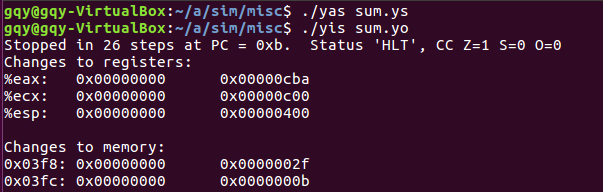
\includegraphics{A_sum}
%		\caption{Part A  {\ttfamily sum.ys}} \label{Part A: sum.ys}%标题 自动编号 label标签
%\end{figure}


%\usepackage{times} % Uncomment to use the Times New Roman font

%----------------------------------------------------------------------------------------
%	DOCUMENT INFORMATION
%----------------------------------------------------------------------------------------

\title{\textbf{操作系统课程设计Project 2\\UNIX Shell Programming\\ \& Linux Kernel Module for Task Information}} % Title

\author{姓名: 郭倩昀  
\\班级: F1903303  
\\学号: 519021910095  
\\Email: guoqianyun@sjtu.edu.cn} % Author name and email
\date{\today} % Date for the report
\begin{document}
\maketitle % Insert the title, author and date
\tableofcontents
\newpage
\section{UNIX Shell Programming}
%\begin{ttfamily}
\subsection{实验内容与目标}
本实验需要利用C语言设计可以接受并执行用户指令的unix shell interface
\begin{itemize}
\item[$\bullet$]创建子进程执行用户指令
\end{itemize}
\subsection{实验过程及步骤}
\begin{itemize}
\item[$\bullet$]指令标准化\\
设计函数void reorganize(char *inst)标准化处理输入的指令,使得其中的空格个数等正常排列不存在特殊的多个空格或者换行情况。
\end{itemize}
\subsection{实验代码}
\begin{center}
{\ttfamily shell.c}
\end{center}
\begin{lstlisting}[language={[ANSI]C}]
# include <stdio.h>
# include <fcntl.h>
# include <stdlib.h>
\end{lstlisting}
\subsection{实验测试}
\begin{itemize}
\item[$\bullet$]shell测试% (图 \ref{shell测试})
%\begin{figure}[htbp]
%		\centering
%		\includegraphics{shell}
%		\caption{shell测试} \label{shell测试}
%\end{figure}

测试指令如下
\begin{lstlisting}[language={[ANSI]C}]
gcc shell.c -o shell
\end{lstlisting}
首先编译shell.c文件并执行,输入!!指令由于历史指令为空报错,之后正常执行ps指令,再输入!!指令就输出了历史指令ps并执行。然后ls -l > tmp和sort < tmp测试输入输出重定位,ls -l | sort测试pipe通信,ls -l \&测试并行。再次执行shell,然后输入ps可以看到当前系统任务列表有两层shell在执行,输入两次exit可以正常退出程序。
\end{itemize}
\section{Conclusion}

\subsection{问题与解决方案}
本次project2的UNIX shell部分稍有一点难度。首先分析指令部分需要对字符串操作比较熟悉;在设计支持重定位和pipe通信的时候遇到了许多新的函数,最开始并没有什么头绪,但是在仔细研读书本示例并经过多次尝试后最终成功完成。

project2的另一个部分pid内核模块的设计是project1延伸,书上的指导也比较细致,就是在设计proc\_write()函数的时候,如果仅仅根据书本上的操作会发现最后pid读取都非法,后来发现需要人为添加字符串结尾字符能避免该问题。

\subsection{实验心得}
本次project2是对所学知识一次很好的运用,比如设计UNIX shell需要有一个全局观念,要综合运用变量设计,空间分配,进程管理等方式,同时在实践的过程中也让我对pipe通信有了更深入的了解。虽然过程中也遇到了一些问题,但在耐心检查反复尝试的过程中都顺利解决了,总的来说本次project很好地锻炼了动手能力并加深了对理论知识的理解,让我受益匪浅。




%----------------------------------------------------------------------------------------


\end{document}